\begin{frame}{Exemple}
    \begin{center}
        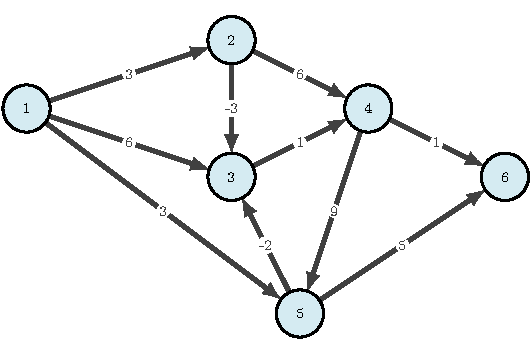
\includegraphics[height=.6\textheight]{fig/bellman-0.pdf}

    \end{center}
\end{frame}

\begin{frame}{Itérations de l'algorithme : itération 1}
    \begin{center}
        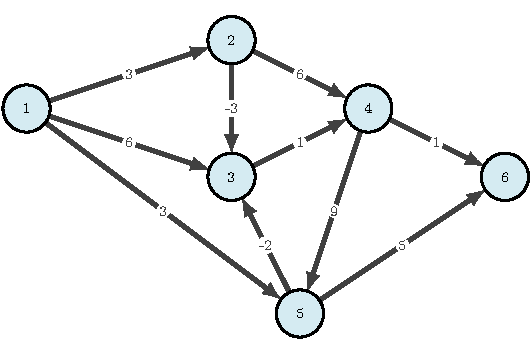
\includegraphics[height=.6\textheight]{fig/bellman-0.pdf}      
    \begin{tabular}{c|cccccc}
      
        & 1    &2      &3      &4      &5      &6      \\
        \hline
        \texttt{pred} & &1      &1      &       &1      &       \\
        \texttt{dist} & 0       &3      &6      &$+\infty$    &3      &$+\infty$    \\

    \end{tabular}
\end{center}
\end{frame}

\begin{frame}{Itérations de l'algorithme : itération 2}
    \begin{center}
        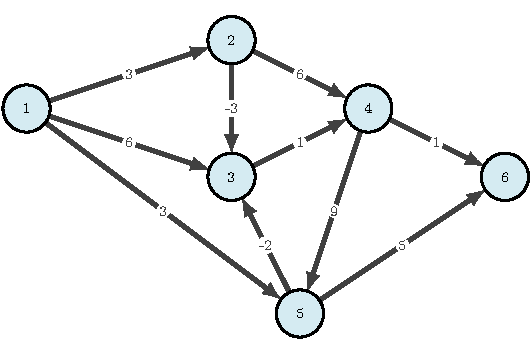
\includegraphics[height=.6\textheight]{fig/bellman-0.pdf}      
    \begin{tabular}{c|cccccc}
      
        & 1    &2      &3      &4      &5      &6      \\
        \hline
        \texttt{pred} & &1      &5      &3      &1      &5           \\
        \texttt{dist} & 0       &3      &1      &7      &3      &8      \\
        
    \end{tabular}
\end{center}
\end{frame}

\begin{frame}{Itérations de l'algorithme : itération 3}
    \begin{center}
        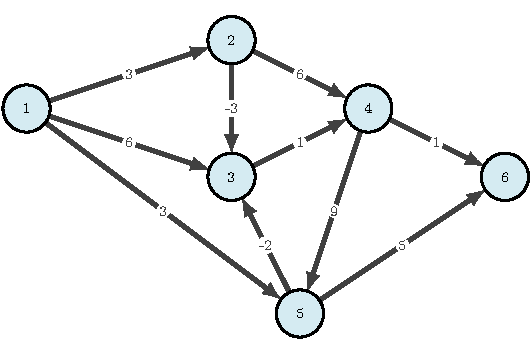
\includegraphics[height=.6\textheight]{fig/bellman-0.pdf}      
    \begin{tabular}{c|cccccc}
      
        & 1    &2      &3      &4      &5      &6      \\
        \hline
        \texttt{pred} & &1      &2      &3      &1      &5      \\
        \texttt{dist} & 0       &3      &0      &2      &3      &8      \\
            \end{tabular}
\end{center}
\end{frame}

\begin{frame}{Itérations de l'algorithme : itération 4}
    \begin{center}
        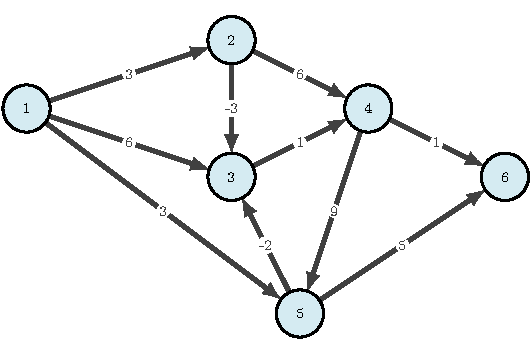
\includegraphics[height=.6\textheight]{fig/bellman-0.pdf}      
    \begin{tabular}{c|cccccc}
      
        & 1    &2      &3      &4      &5      &6      \\
        \hline
        \texttt{pred} & &1      &2      &3      &1      &4      \\
        \texttt{dist} & 0       &3      &0      &1      &3      &3      \\
                    \end{tabular}
\end{center}
\end{frame}


\begin{frame}{Itérations de l'algorithme : itération 5}
    \begin{center}
        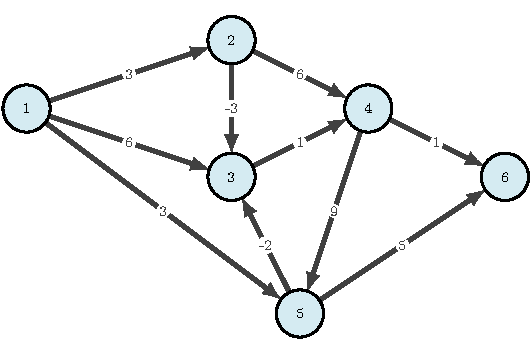
\includegraphics[height=.6\textheight]{fig/bellman-0.pdf}      
    \begin{tabular}{c|cccccc}
      
        & 1    &2      &3      &4      &5      &6      \\
        \hline
        \texttt{pred} & &1      &2      &3      &1      &4     \\
        \texttt{dist} & 0       &3      &0      &1      &3      &2 \\                    \end{tabular}
\end{center}
\end{frame}

